%!TEX root=../../autopilot.tex
\section{GPIO Latency}
\label{sec:gpiolatency}

Neurons compute at millisecond timescales, so any task that links neural computation to behavior needs to have near-millisecond latency. We start by characterizing Autopilot's GPIO control latency in "script mode" --- using the GPIO control classes on their own, without using any of the rest of Autopilot's modules.

\begin{margintable}[0.5cm]
\caption{GPIO Latency Materials. (Parameters in \{\} are input in separate runs)}
\label{tab:gpiomaterials}
\noindent\begin{tabularx}{\linewidth}{lX}%
\toprule
\textbf{Code} & \href{https://github.com/auto-pi-lot/plugin-paper/blob/main/plugin_paper/scripts/test_gpio.py}{test\_gpio.py} \\
\textbf{replicate} & \texttt{python test\_gpio.py -w \{0,1,2\} -n 100000}\\
\textbf{gpiozero} & \href{https://github.com/auto-pi-lot/plugin-paper/blob/main/plugin_paper/hardware/zero.py}{1.6.2} \\
\textbf{pigpio} & \href{https://github.com/sneakers-the-rat/pigpio/commit/3c237159e5995ec58cd673579bdd66a8d819b269}{3c23715} \\
\bottomrule
\end{tabularx}
\end{margintable}

\subsection{Output Latency}

We first tested the software measured latency between when a command to write a value to a GPIO pin is issued and when it completes (Figure \ref{fig:gpiolags}, Table \ref{tab:gpiomaterials}). By default, the pigpio interface we use to control GPIO pins issues a command and then confirms the request was successful by querying the pigpio daemon for the status of the pin (Write+Read). We \href{https://github.com/sneakers-the-rat/pigpio/commit/0782de06f0a5c092063118733ad2df9d65f1f1a0}{extended} pigpio to just issue the command without confirmation to estimate the true time between when the command is issued and when the voltage of the pin changes (Write). Each of these operations takes roughly 40$\mu s$ with minimal jitter (Median $\pm$ IQR --- Write Only: 40.8$\mu s \pm$0.41, Write and Read: 88.4 $\mu s \pm$2.02, n=100,000 each).

\begin{figure}[hb!]
\caption{Software latency from GPIO write to completion of command. Values are presented as medians $\pm$ IQR with n=100,000 tests for each. A random subsample of 500 (for tractability of plotting) of each type of test are presented (black points) after filtering to the bottom 99th percentile to exclude extreme outliers.  Commands sent using pigpio (red) took roughly 40$\mu s$ each (write and read are effectively two separate commands, Write Only: 40.8$\mu s \pm$0.41, Write and Read: 88.4 $\mu s \pm$2.02). The prototype gpiozero wrapper (blue) using RPi.GPIO as its backend was faster, taking 16.2$\mu s \pm$0.22 to complete.}
\label{fig:gpiolags}
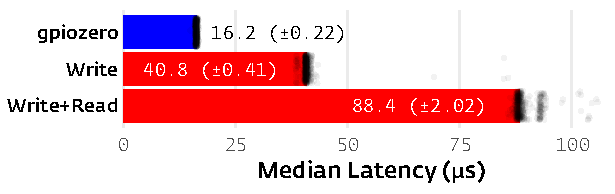
\includegraphics{autopilot/autopilot/src/figures/gpio_latency_small.pdf}
\end{figure}

Pigpio is useful as a general purpose controller because of its ability to run scripts within its daemon, use hardware PWM via direct memory access, and consistently poll for pin state, but takes a latency penalty because the python interface communicates with it through a local TCP socket. To demonstrate the flexibility of Autopilot in incorporating additional software libraries, we wrote a \href{https://github.com/auto-pi-lot/plugin-paper/blob/main/plugin_tests/hardware/zero.py}{thin wrapper} around \href{https://gpiozero.readthedocs.io/en/stable/}{gpiozero}, which can use \href{https://pypi.org/project/RPi.GPIO/}{RPi.GPIO} to directly write to the GPIO registers. For simple output, this wrapper proved to be faster (16.2 $\mu s \pm 0.22$, n=100,000), and with \~63 lines of code is now available in the plugin accompanying this paper to be used, repurposed, and extended.

\subsection{Roundtrip Input/Output Latency}

\begin{margintable}[2cm]
\caption{Roundtrip Latency Materials}
\label{tab:roundtrip}
\noindent\begin{tabularx}{\linewidth}{lX}%
\toprule
\textbf{Function Generator} & \href{https://wiki.auto-pi-lot.com/index.php/Koolertron\_CJDS98}{Koolertron CJDS98} \\
\textbf{Code} & \href{https://github.com/auto-pi-lot/plugin-paper/blob/main/plugin_paper/scripts/test\_gpio.py}{test\_gpio.py} \\
\textbf{Replicate} & \texttt{python test\_gpio.py -w \{3,4\}} \\
\bottomrule
\end{tabularx}
\end{margintable}


Output commands usually aren't issued in isolation, but as a response to some external or task-driven trigger. We measured the roundtrip latency from a 5V square pulse from an external function generator to when an output pin was flipped from low to high on an oscilloscope (Table \ref{tab:roundtrip}). 

Typically that is as much methodological detail as you would expect in a scientific paper, but actually making those measurements via oscilloscope requires knowing how to set up such a test as well as how to extract the measured data afterwards --- which is not altogether trivially available technical knowledge. As an example of how integrating semantically linked documentation with experimental tools enables a fundamentally deeper kind of reproducibility and methodological transparency, we instead documented these operations, including a code sample and a guide to unlocking additional features on our oscilloscope on the \href{https://wiki.auto-pi-lot.com/index.php/Rigol\_DS1054Z}{autopilot wiki}. The code to extract traces from the oscilloscope is also included in this paper's \href{https://wiki.auto-pi-lot.com/index.php/Plugin:Autopilot\_Paper}{plugin}, which links to the oscilloscope page with a \texttt{[[Controls Hardware::Rigol DS1054Z]]} tag, so it is possible to bidirectionally find code examples from the oscilloscope page as well as find further documentation about the hardware used in this paper from the plugin page. The same can be true for any hardware used by any plugin in any paper using Autopilot.

We used the \texttt{assign\_cb} method of the \href{https://docs.auto-pi-lot.com/en/latest/hardware/gpio.html\#autopilot.hardware.gpio.Digital_In.assign_cb}{\texttt{Digital\_In}} class to test the typical roundtrip latency that Autopilot objects can deliver. This gave us a median 474 $\mu s$ (IQR: 52.5$\mu s$) latency (Red in Figure \ref{fig:gpiort}). GPIO callbacks are flexible, and can use arbitrary python functions, but if all that's needed is to trigger one pin off of another with some simple logic like a parametric digital waveform or static "on" time, pigpio also allows us to directly program pin to pin logic as a "\href{http://abyz.me.uk/rpi/pigpio/pigs.html}{pigs}" script (literally Figure \ref{fig:pigsscript}) that runs within the pigpio daemon. The pigs script gave us roughly three orders of magnitude lower latency (Median $\pm$ IQR: 370ns $\pm$ 140, blue in \ref{fig:gpiort}). 

\begin{marginfigure}[-10cm]
\begin{pythoncode*}{
label= \texttt{Pigs Trigger Script},
frame=lines,
linenos=false}
" ".join([
  "tag 999",
  # read input pin
  f"r {pin_in.pin_bcm}",
  # if off, goto 998
  f"jz 998", 
  # else, turn on
  f"w {pin_out.pin_bcm} 1",
  # then goto 999
  "jp 999", 
  "tag 998",
  # turn off
  f"w {pin_out.pin_bcm} 0",
  # jump to beginning
  f"jp 999"
])
\end{pythoncode*}
\caption{The pigs script used to trigger one pin (pin\_out), from another (pin\_in). At the expense of a little bit of complexity having to write a script in its scripting language, we are able to reduce latency by three orders of magnitude.}
\label{fig:pigsscript}
\end{marginfigure}


\begin{figure}[hb!]
\caption{Roundtrip latency from external trigger to digital output using two methods: Typical Autopilot callback function given to a \texttt{Digital\_In} object that turns a \texttt{Digital\_Out} pin on for 1ms when an input pin changes state (Red, Left, Median $\pm$ IQR: 474 $\mu s \pm$ 52.5). Pigs script that runs entirely within the pigpio daemon (Blue, Right, 380ns $\pm$ 140). For each, black points represent individual measurements (n=525), annotations are quartiles.}
\label{fig:gpiort}
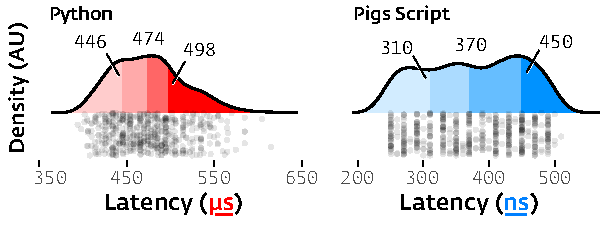
\includegraphics{autopilot/autopilot/src/figures/gpio_roundtrip_density.pdf}
\end{figure}

\clearpage


